\section{Digital filtrering}
Der findes to former for digital filtrering; Infinite Impulse Response (IIR) og Finite Impulse Response (FIR). Der ses hertil både fordele og ulemper ved begge filtertyper \citep{blandford2012}.

FIR-filtre kan altid laves, således de har en lineær fase, og de er altid stabile. FIR-filtre designes ved at benytte eksempelvis frekvenssampling eller en bestemt vindue-type, hvilket giver en overførselsfunktion. Denne overførselsfunktion kan herved benyttes som digitalt filter \citep{blandford2012}. 

I modsætning til FIR-filtre, har IIR-filtre ikke en lineær fase, og de kan være ustabile. Ud over dette har IIR-filtre stejlere sidelobes end et IIR-filter med samme antal koefficienter. Dette betyder, at filteret er mindre hukommelseskrævende og kan arbejde hurtigere. IIR-filtres designprocedure er udledt af den procedure, som de analoge filtre er designet efter. Af denne grund laves IIR-filtre, ligesom analoge filtre, som Butterworth, Chebyshev type 1 og 2 og elliptiske filtre \citep{blandford2012}. Disse er illustreret på \autoref{fig:filtre}. 
\\

\begin{figure}[H]
\centering
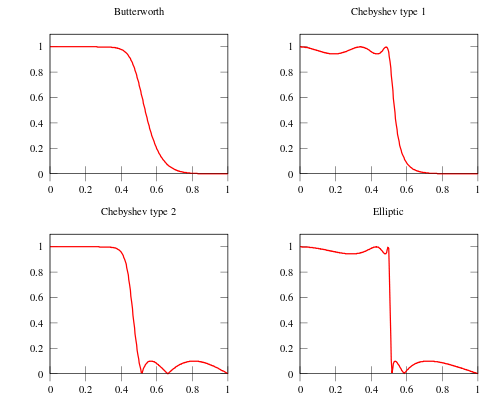
\includegraphics[width=0.6\textwidth]{figures/filtre}
\caption{De fire filtertyper; Butterworth, Cehbyshev 1 \& 2 og elliptisk \citep{wikipedia2016}}
\label{fig:filtre}
\end{figure}

Et Butterworth filter er karakteriseret ved ikke at have nogle rippels i hverken pasbåndet eller stopbåndet. Hertil er der, uanset filterorden, en dæmpning på 3 dB ved knækfrekvensen \citep{nilsson2015}.
Et Chebyshev filter har i modsætning til Butterworth et kortere transitionsbånd, som følge af en stejlere dæmpning, dog forekommer der ved et Chebyshev filter enten rippels i pasbåndet eller i stopbåndet. Ved et type 1 Chebyshev filter ses rippels i pasbåndet samt en monotont variation i stopbåndet. For type 2 Chebyshev ses der derimod rippels i stopbåndet og en monotont variation i pasbåndet \citep{nilsson2015}. 
Ved det elliptiske filter ses en endnu stejlere dæmpning og dermed et kortere transitionsbånd end ved Butterworth samt Chebyshev filtre. Ved dette filter ses der dog både rippels i pasbånd og stopbånd \citep{nilsson2015}. 


Da der ønskes at frafiltrere lavfrekvent støj fra det forstærkede, ensrettede og lavpasfiltrerede EMG-signal, vil et IIR højpasfilter være fordelagtigt for at opnå en skarpere hældning i transitionsbåndet. Herudover vil implementering af et FIR-filter kræve for meget af PSoC'en. Under pilotforsøget i \autoref{sec:pilotforsoeg} ... \fxnote{Dette afsnit skal ændres i forhold til hvilket filter vi anvende til henholdsvis accelerometer og EMG}

\subsubsection{Filter: accelerometer}
\begin{itemize}
\item Signalet skal være 
\item Skal have en knækfrekvens på $XX~Hz$
\item Skal have et stopbånd på $XX~Hz$
\item Skal have en minimumsdæmpning på $XX~dB$
\item Skal anvende et filter med en knækfrekvens på $XX~Hz$
\end{itemize}

\subsubsection{Filter: EMG}
\begin{itemize}
\item Skal have en knækfrekvens på $XX~Hz$
\item Skal have et stopbånd på $XX~Hz$
\item Skal have en minimumsdæmpning på $XX~dB$
\item Skal anvende et filter med en knækfrekvens på $XX~Hz$
\end{itemize}